\documentclass[aps, secnumarabic, balancelastpage, asmath, amssymb, nofootinbib, floatfix,]{revtex4-2}
\usepackage[titles]{tocloft}
\usepackage[newfloat]{minted}
\usepackage{graphicx}
\usepackage{float}
\usepackage{caption}
\usepackage{siunitx}
\usepackage[export]{adjustbox}
\usepackage{subcaption}
\usepackage{amsmath}
\usepackage{hyperref}
\usepackage{subcaption}
\usepackage{tikz}
\usepackage{multirow}
% \usepackage[table,xcdraw]{xcolor}
\usepackage{xcolor}
\usepackage{cprotect}
\usepackage{verbatimbox}
\usepackage{listings}
\usepackage{xparse}
\usepackage{listings}
\usepackage{paralist}
\usepackage[export]{adjustbox}
\usepackage{svg}
\usepackage{xurl}
%\usepackage{times}
\NewDocumentCommand{\codeword}{v}{%
\texttt{\textcolor{black}{#1}}%
}

\hypersetup{colorlinks=true, pdfstartview=FitV, linkcolor=blue, citecolor=black, plainpages=false, pdfpagelabels=true, urlcolor=black}

\newenvironment{code}{\captionsetup{type=listing}}{}
\SetupFloatingEnvironment{listing}{name=Source Code}

\definecolor{backcolour}{rgb}{0.95,0.95,0.92}
\definecolor{mGreen}{rgb}{0,0.6,0}
\definecolor{mGray}{rgb}{0.5,0.5,0.5}
\definecolor{mPurple}{rgb}{0.58,0,0.82}
\definecolor{backgroundColour}{rgb}{0.95,0.95,0.92}
\definecolor{LightGray}{gray}{0.9}

\setlength{\arrayrulewidth}{0.3mm}
\setlength{\tabcolsep}{5pt}
\renewcommand{\arraystretch}{1.5}
\graphicspath{{./image/}}

\usepackage{setspace}
\usepackage{titletoc}
%\contentsmargin{2.55em}
\dottedcontents{chapter}[1.5em]{}{2.3em}{1pc}
\dottedcontents{section}[1.5em]{}{1.7em}{0.5pc}
\dottedcontents{subsection}[3.9em]{}{2.4em}{0.5pc}
\dottedcontents{subsubsection}[6.6em]{}{2.7em}{0.5pc}
\dottedcontents{paragraph}[10.2em]{}{3.5em}{0.5pc}

\usepackage{etoolbox}
\makeatletter
\pretocmd{\chapter}{addtocontents{toc}{\protect\addvspace{15\p@}}}{}{}
\pretocmd{\section}{\addtocontents{toc}{\protect\addvspace{9\p@}}}{}{}
%\pretocmd{\subsection}{\addtocontents{toc}{\protect\addvspace{15\p@}}}{}{}
\makeatother


\stepcounter{secnumdepth}
\stepcounter{tocdepth}

% Usual (decimal) numbering
\renewcommand{\thesection}{\arabic{section}}
\renewcommand{\thesubsection}{\thesection.\arabic{subsection}}
\renewcommand{\thesubsubsection}{\thesubsection.\arabic{subsubsection}}

% Fix references
\makeatletter
\renewcommand{\p@subsection}{}
\renewcommand{\p@subsubsection}{}
\makeatother

\lstset
{ %Formatting for code in appendix
    basicstyle=\footnotesize,
    numbers=left,
    stepnumber=1,
    showstringspaces=false,
    tabsize=1,
    breaklines=true,
    breakatwhitespace=false,
    %basicstyle=\ttfamily,
    %columns=fullflexible,
    frame=single,
    postbreak=\mbox{\textcolor{red}{$\hookrightarrow$}\space},
    numbersep=5pt,
}

\def\bibsection{\section*{\refname}}
\usepackage{wrapfig}
\usepackage{relsize}
\usepackage{epstopdf}
\usepackage{booktabs}

\def\justifying{%
  \rightskip=0pt
  \spaceskip=0pt
  \xspaceskip=0pt
  \relax
}

% \usepackage{listings}
% \usepackage{listing}
% \renewcommand\listoflistingscaption{List of source codes}

\begin{document}
%top matter
    \begin{titlepage}
   \begin{center}
       \vspace*{1cm}

	\Huge
       \textbf{CE323 - Advanced Embedded Systems Design}

       \vspace{0.5cm}

       \LARGE
        \textbf{Assignment Report\\Home Alarm System}

       \vspace{1.5cm}

       \textbf{Akshay Gopinath}\\
       \textbf{Registration Number: 2005614}

   \end{center}
   \tableofcontents
   \listoffigures


\end{titlepage}

%\thispagestyle{plain}
%\Large
%\textbf{Contributions}

%\clearpage

% \thispagestyle{plain}
% \begin{center}
%     \Large
%     \textbf{CE315 - Mobile Robotics}

%     \vspace{0.4cm}
%     \large
%     \textbf{Assignment 1 Report}

%     \vspace{0.4cm}
%     \textbf{Akshay Gopinath}

%     %\vspace{0.9cm}
%     \section*{Abstract}
%     \fontsize{11pt}{12pt}\selectfont

% \end{center}
% \fontsize{11pt}{12pt}\selectfont
% {
% \setlength{\parindent}{0pt}

% {\bf Insert Abstract here}

% }
% \clearpage

% \tableofcontents

%\clearpage

% \listoffigures
% \clearpage

% \listoftables

\clearpage


\section{\fontsize{11.3pt}{12pt}\selectfont \bf Introduction}
\fontsize{11pt}{12pt}\selectfont
\label{sec:1}

{
\setlength{\parindent}{0pt}

This report documents a design of a home alarm system on an Embedded platform. The target embedded device is the ARM mbed LPC1768 development board which houses a 32-bit Cortex-M3 Microcontroller. The software design used is scheduler based, where tasks are configured to run at set refresh rates, allowing for clean, extendable, modular and flexible code.

\subsection{\fontsize{11.4pt}{12pt}\selectfont \bf Requirments Form \label{sec:1.1}}
\setlength{\parindent}{0pt}
{
% \Large
{\bf Name: }Home Alarm System
~\\
~\\
{\bf Purpose: }To prevent uninvited house intrusion by detecting sensor activation within the various zones.
~\\
~\\
{\bf Inputs: }Keypad to enter password, Normally Open/Closed sensors/switches at each zone.
~\\
~\\
{\bf Outputs: }LED to display the system status, LCD screen for user interface.
~\\
~\\
{\bf Function Specifications: }The system has 6 states, unset, exit, set, entry, alarm and report. 
\begin{itemize}
\item \textbf{Unset State: }Activation of sensors should not cause the alarm LED to blink, and entry of the correct passcode will cause a transition to the set state. Entry of wrong passcode will transition to alarm state.
\item \textbf{Exit State: }There is a configurable time interval (exit period) for example 1 minute for evacuation. The alarm LED will be blinking. Entry of correct passcode will transition back to unset state. Transition to alarm state occurs when incorrect code is entered three times or if any sensor is activated. If all sensors are inactive after the exit period expires, the system transitions to the entry state.
\item \textbf{Set State: }Activation of entry/exit zone sensor causes a transition to the entry state. Activation of other sensors will make the system transition to the alarm state.
\item \textbf{Entry State: }The entry period is a configurable time limit, for example 1 minute. The alarm LED will blink. The correct passcode will change the system back to unset state. Activation of any sensor or if the correct password is not entered within the time limit, the system transitions to the alarm state.
\item \textbf{Alarm State: }Alarm LED should be on all the time and switch off after 2 minutes. If incorrect password is entered, the system stays in alarm state, else it transitions to report state.
\item \textbf{Report State: }The LCD screen displays which zones have been triggered (the error code). And the system can be cleared (transition back to unset state) when the enter button is pressed.
\end{itemize}
~\\
{\bf Performance: }The tasks refresh rates in the system have been tuned for optimal performance. The is LCD updated every 200ms, the keypad polling refresh rate is set to 100ms. The sensor/switch task is ran at a rate of 100ms.
~\\
~\\
{\bf Manufacture costs: }Less than £100 including the Microcontroller, LCD screen, keypad and sensors/switches.
~\\
~\\
{\bf Physical size/weight: }The sensors/switches should be sized well to comfortably fit into doors and windows. The user interface (keyboard and LCD) should fit on a house dashboard.
~\\
~\\
{\bf Project Constraints: }Due to the hardware available, switches will represent sensor activation and an LED will represent the alarm. Figure \ref{fig:appendix1} in the appendix shows the hardware used for the project.
~\\
~\\
{\bf Design Parameters: }The software has various configurable paramaters such as exit state and entry state time limit, LCD refresh rate and Keypad poll rate, alarm state LED on time, password, sensor poll rate.


}

\clearpage

\section{\fontsize{11.3pt}{12pt}\selectfont \bf State Machine Diagram}
\fontsize{11pt}{12pt}\selectfont
\label{sec:2}

\begin{figure}[h]
  \centering
  %\captionsetup{justification=centering}
  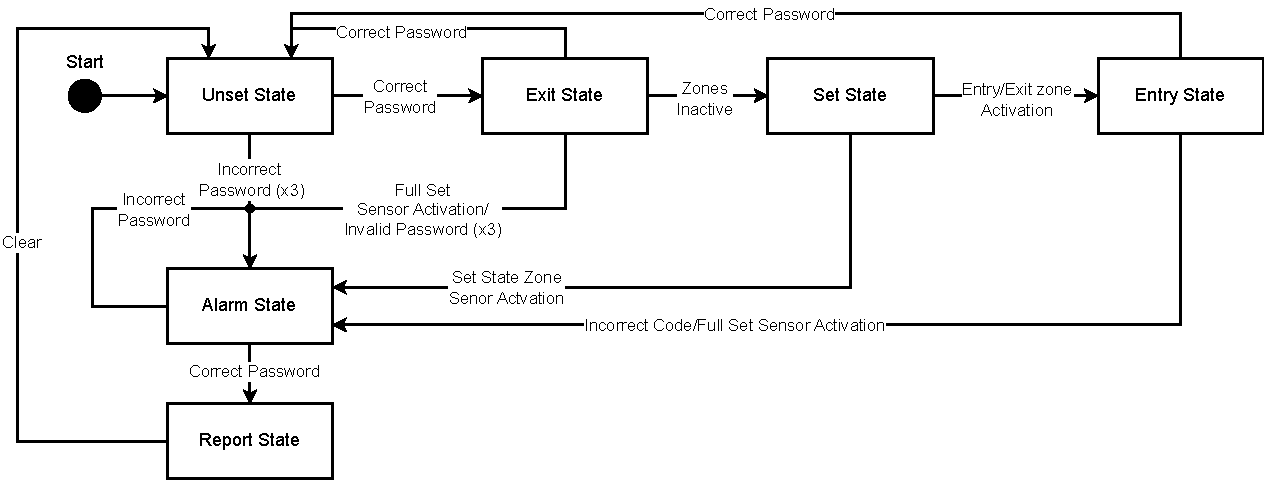
\includegraphics[scale = 0.85]{ce323-state-diagram.pdf}
  \caption{\em State Machine Diagram}
  \label{fig:image1}
\end{figure}

Figure \ref{fig:image1} above represents the state machine diagram of the home alarm system. The system has 6 states, which are: Unset State, Exit State, Set State, Entry State, Alarm State, Report State. The starting state is the Unset state. Since the system always loops back to the Unset State, there is no ending state. \\
\\
In the Unset State, the system will not react to any sensor activation. If the wrong password is entered three times, the system jumps to the alarm state. The entry of the correct four digit password will result in a transition to the Exit State. \\

During the Exit State, the user has an `exit period' during which they can evacuate their home. The entry period in the software is set to one minute, and is configurable in the code. The system changes to a different state depending on certain conditions. If any of the eight sensors is activated, the alarm system will jump to the alarm state, and also if the incorrect password is entered three times. Within the exit period, if the correct password is entered, the system transitions back to the unset state. If the exit period expires and all sensors are inactive, the system enters the set state. The alarm LED will be blinking in this state.\\
\\
Within the set state, if the entry/exit zone sensor is activated, the system enters the Entry State, else if any of the other 7 sensors is activated, the system will move to the Alarm State.\\
\\
In the Entry State, there is a period of time when the user can gain access to their home, so that the user can unset the alarm. The `entry period' (the time limit) is set to one minute, which is also configurable in the code. If the correct 4 digit passcode is entered, the system transitions back to the unset state. The system enters the alarm state under two conditions. The first when the user fails to enter the correct password within in the time limit. The second when the any of the sensors are activated. In this state, the alarm LED is blinking.\\
\\
In the alarm state, the alarm LED is on all the time and after 2 minutes, it switches off. If the correct password is entered, the system enters the report state, else it stays in the alarm state.\\
\\
In the report state, the LCD shows the error code. The error code can either be the zone numbers where the sensors were triggered, or the incorrect password. And the user can clear the system by pressing a button on the keypad. Once the system is cleared, the system moves back to the starting state, which is the Unset State.


\clearpage

\section{\fontsize{11.3pt}{12pt}\selectfont \bf Class Diagram}
\fontsize{11pt}{12pt}\selectfont
\label{sec:3}


\begin{figure}[h]
  \centering
  %\captionsetup{justification=centering}
  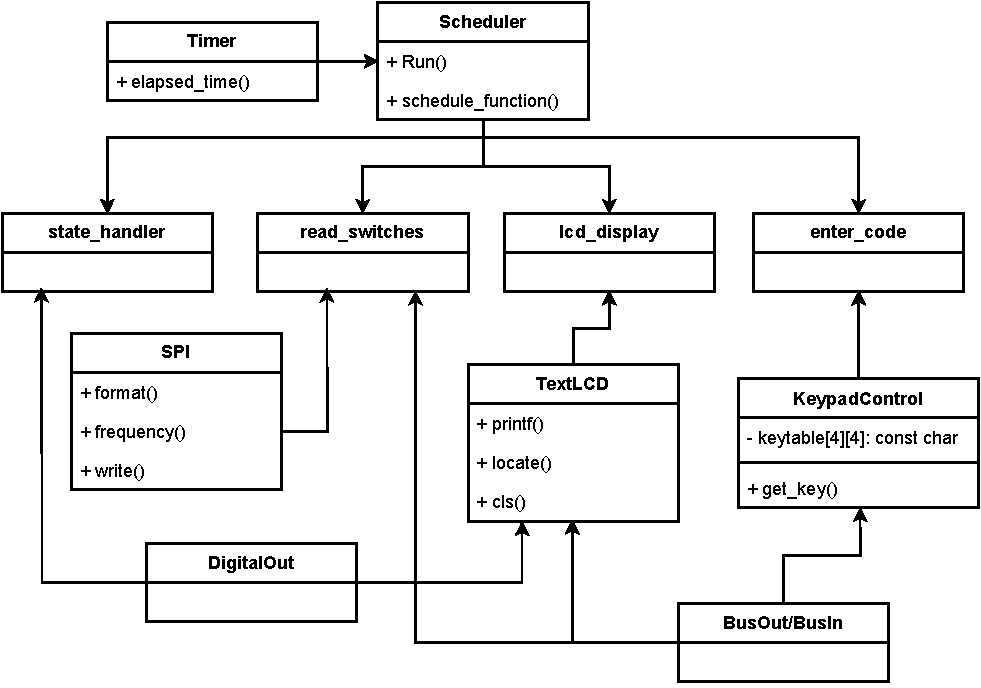
\includegraphics[scale = 1.08]{class.drawio.pdf}
  \caption{\em Class Diagram}
  \label{fig:image2}
\end{figure}

Figure \ref{fig:image2} above shows the class dependency diagram for the home alarm system. The main heart of the software is the \verb|Scheduler| class, which controls and runs all the operations of the system (for example displaying to LCD). The scheduler class depends on the internal timer of the mbed, which is implemented by the \verb|Timer| class. The \verb|Timer| class is provided by the mbed framework library. The Scheduler controls four free form functions: \verb|state_handler|, \verb|read_switches|, \verb|lcd_display| and \verb|enter_code|. Since these methods act independently because of the scheduler, they are treated like objects for this diagram. The \verb|state_handler| task depends on the \verb|DigitalOut| class from the mbed framework, as the \verb|state_handler| also controls the alarm LED. The \verb|read_switches| task depends on \verb|SPI|, \verb|BusOut| and \verb|BusIn|. The \verb|BusOut| class is used as the chip select to select the switches and \verb|BusIn| is used to receive the switch readings. Serial Peripheral Interface (SPI) protocol is used to communicate with the red/green LEDs on the hardware which is set according to the current switch reading.\\
The \verb|TextLCD| library is a third party library to drive the LCD. \verb|TextLCD| inherits of a class called \verb|Stream| which is an internal class in the mbed framework to handle standard input and output (\verb|stdin| and \verb|stdout|). This library also depends on \verb|BusOut|, \verb|BusIn| and \verb|DigitalOut|. The \verb|lcd_display| task depends on the \verb|TextLCD| library.\\
The \verb|KeypadControl| class was created to drive the keypad on the hardware for user input. And this class also depends on the \verb|BusOut| and \verb|BusIn| from the mbed library. The \verb|enter_code| task uses the \verb|KeypadControl| class object to take user input.

\clearpage

\section{\fontsize{11.3pt}{12pt}\selectfont \bf Sequence Diagram}
\fontsize{11pt}{12pt}\selectfont
\label{sec:4}

\begin{figure}[h]
  \centering
  %\captionsetup{justification=centering}
  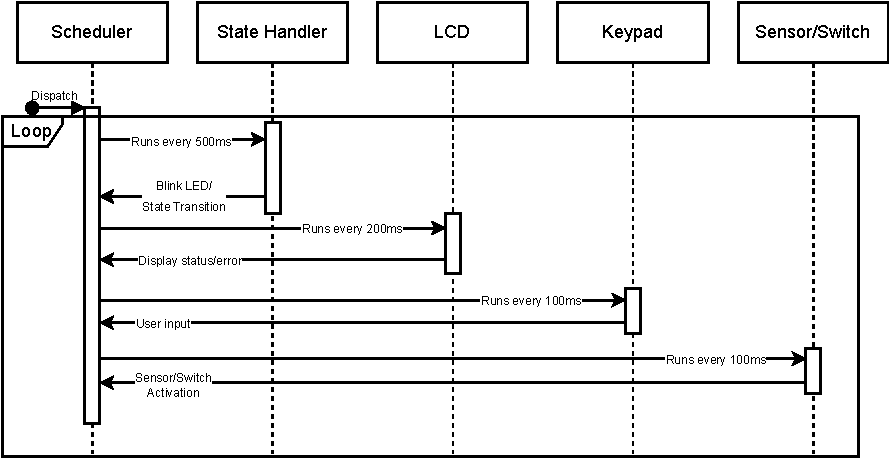
\includegraphics[scale = 1.2]{seq.drawio.pdf}
  \caption{\em Sequence Diagram}
  \label{fig:image3}
\end{figure}

Figure \ref{fig:image3} above shows the sequence diagram of the home alarm system. The sequence diagram depicts the order and timeline of the system behaviour. Since the software design is based on a task based scheduling system, the sequence diagram is represented by the individual tasks that are spun in the main scheduling loop. The running tasks are placed in the order at which they are initialised and run in the sequence diagram, with respect to the scheduler. The length of the bar on the lifeline for each task is dependent on the frequency at which the function is called. Lower the frequency at which it is called in (a loop), the lower the active time of the task on the lifeline. And every task in the scheduler is run continuously, essentially in a loop.~\\
As seen in Figure \ref{fig:image3} above, the tasks are initialised and run in the order: State Handler, LCD, Keypad, Sensor/Switch, one by one in a scheduled loop. The task that is run the least frequently is the state handler, hence has the highest active time. This task is run every 500ms. The State Handler task controls the alarm LED as well as any state transition that are time sensitive. The next task in the order, LCD, is run every 200ms. This task is responsible for displaying error and status messages to the user. The next two tasks (in order: Keypad, Sensor/Switch) have the same frequency of 100ms. These two tasks are run at the highest frequency as performance is critical here. The keypad is used for the user input and hence must be responsive. As for the Sensor/Switch task, the system needs to be able to detect a sensor activation as well toggle the sensor LED (between red and green) as fast as possible.~\\
Each task after it is run (and the method has finished it's execution cycle) will return to the Scheduler so that the next scheduled task can be run.



\clearpage

\section{\fontsize{11.3pt}{12pt}\selectfont \bf Appendix}
\fontsize{11pt}{12pt}\selectfont
\label{sec:5}

\begin{listing}[!ht]
\caption{main.cpp}
\inputminted[
frame=single,
framesep=10pt,
baselinestretch=1.2,
bgcolor=backgroundColour,
fontsize={\fontsize{8.5}{6.5}\selectfont},
linenos,
tabsize=2,
% breaklines
]
{cpp}{../src/main.cpp}
\label{listing:1}
\end{listing}

\begin{listing}[!ht]
\caption{main.h}
\inputminted[
frame=single,
framesep=10pt,
baselinestretch=1.2,
bgcolor=backgroundColour,
fontsize={\fontsize{8.5}{6.5}\selectfont},
linenos,
tabsize=2,
% breaklines
]
{cpp}{../src/main.h}
\label{listing:2}
\end{listing}

\clearpage

\begin{listing}[!ht]
\caption{keypad\_control.cpp}
% \vspace{-1em}
\inputminted[
frame=single,
framesep=10pt,
baselinestretch=1.2,
bgcolor=backgroundColour,
fontsize={\fontsize{8.5}{6.5}\selectfont},
linenos,
tabsize=2,
% breaklines
]
{cpp}{../src/keypad_control.cpp}
\label{listing:3}
\end{listing}

% \vspace{-3em}
\begin{listing}[!ht]
\caption{keypad\_control.h}
% \vspace{-1em}
\inputminted[
frame=single,
framesep=10pt,
baselinestretch=1.2,
bgcolor=backgroundColour,
fontsize={\fontsize{8.5}{6.5}\selectfont},
linenos,
tabsize=2,
% breaklines
]
{cpp}{../src/keypad_control.h}
\label{listing:4}
\end{listing}

\clearpage

\begin{listing}
\caption{initialisation.cpp}
\vspace{-1em}
\inputminted[
frame=single,
framesep=10pt,
baselinestretch=1.2,
bgcolor=backgroundColour,
fontsize={\fontsize{8.5}{6.5}\selectfont},
linenos,
tabsize=2,
% breaklines
]
{cpp}{../src/initialisation.cpp}
\label{listing:5}
\end{listing}

% \clearpage
\begin{listing}
\caption{initialisation.h}
\inputminted[
frame=single,
framesep=10pt,
baselinestretch=1.2,
bgcolor=backgroundColour,
fontsize={\fontsize{8.5}{6.5}\selectfont},
linenos,
tabsize=2,
% breaklines
]
{cpp}{../src/initialisation.h}
\label{listing:6}
\end{listing}

\clearpage

\begin{listing}[!ht]
\caption{system.h}
\inputminted[
frame=single,
framesep=10pt,
baselinestretch=1.2,
bgcolor=backgroundColour,
fontsize={\fontsize{8.5}{6.5}\selectfont},
linenos,
tabsize=2,
% breaklines
]
{cpp}{../src/system.h}
\label{listing:1}
\end{listing}

\clearpage

\begin{listing}[!ht]
\caption{tasks.h}
\inputminted[
frame=single,
framesep=10pt,
baselinestretch=1.2,
bgcolor=backgroundColour,
fontsize={\fontsize{8.5}{6.5}\selectfont},
linenos,
tabsize=2,
% breaklines
]
{cpp}{../src/tasks.h}
\label{listing:1}
\end{listing}

% \clearpage

% \begin{listing}[h]
% \caption{ Example from external file}
\begin{code}
\captionof*{listing}{ Source Code 9: {task.cpp}}
\inputminted[
frame=single,
framesep=10pt,
baselinestretch=1.2,
bgcolor=backgroundColour,
fontsize={\fontsize{8.5}{6.5}\selectfont},
linenos,
tabsize=2,
% breaklines
]
{cpp}{../src/tasks.cpp}
\label{listing:1}
\end{code}
% \end{listing}

% \clearpage
\begin{code}
\captionof*{listing}{ Source Code 10: {scheduler.cpp}}
\inputminted[
frame=single,
framesep=10pt,
baselinestretch=1.2,
bgcolor=backgroundColour,
fontsize={\fontsize{8}{6.5}\selectfont},
linenos,
tabsize=2,
% breaklines
]
{cpp}{../src/scheduler.cpp}
\label{listing:1}
\end{code}

\clearpage
\begin{code}
\captionof*{listing}{ Source Code 11: {scheduler.h}}
\inputminted[
frame=single,
framesep=10pt,
baselinestretch=1.2,
bgcolor=backgroundColour,
fontsize={\fontsize{8.5}{6.5}\selectfont},
linenos,
tabsize=2,
% breaklines
]
{cpp}{../src/scheduler.h}
\label{listing:1}
\end{code}

\clearpage
\begin{code}
\captionof*{listing}{ Source Code 12: {pin\_map.h}}
\inputminted[
frame=single,
framesep=10pt,
baselinestretch=1.2,
bgcolor=backgroundColour,
fontsize={\fontsize{8.5}{6.5}\selectfont},
linenos,
tabsize=2,
% breaklines
]
{cpp}{../src/pin_map.h}
\label{listing:1}
\end{code}

\clearpage

\begin{figure}[h]
  \centering
  %\captionsetup{justification=centering}
  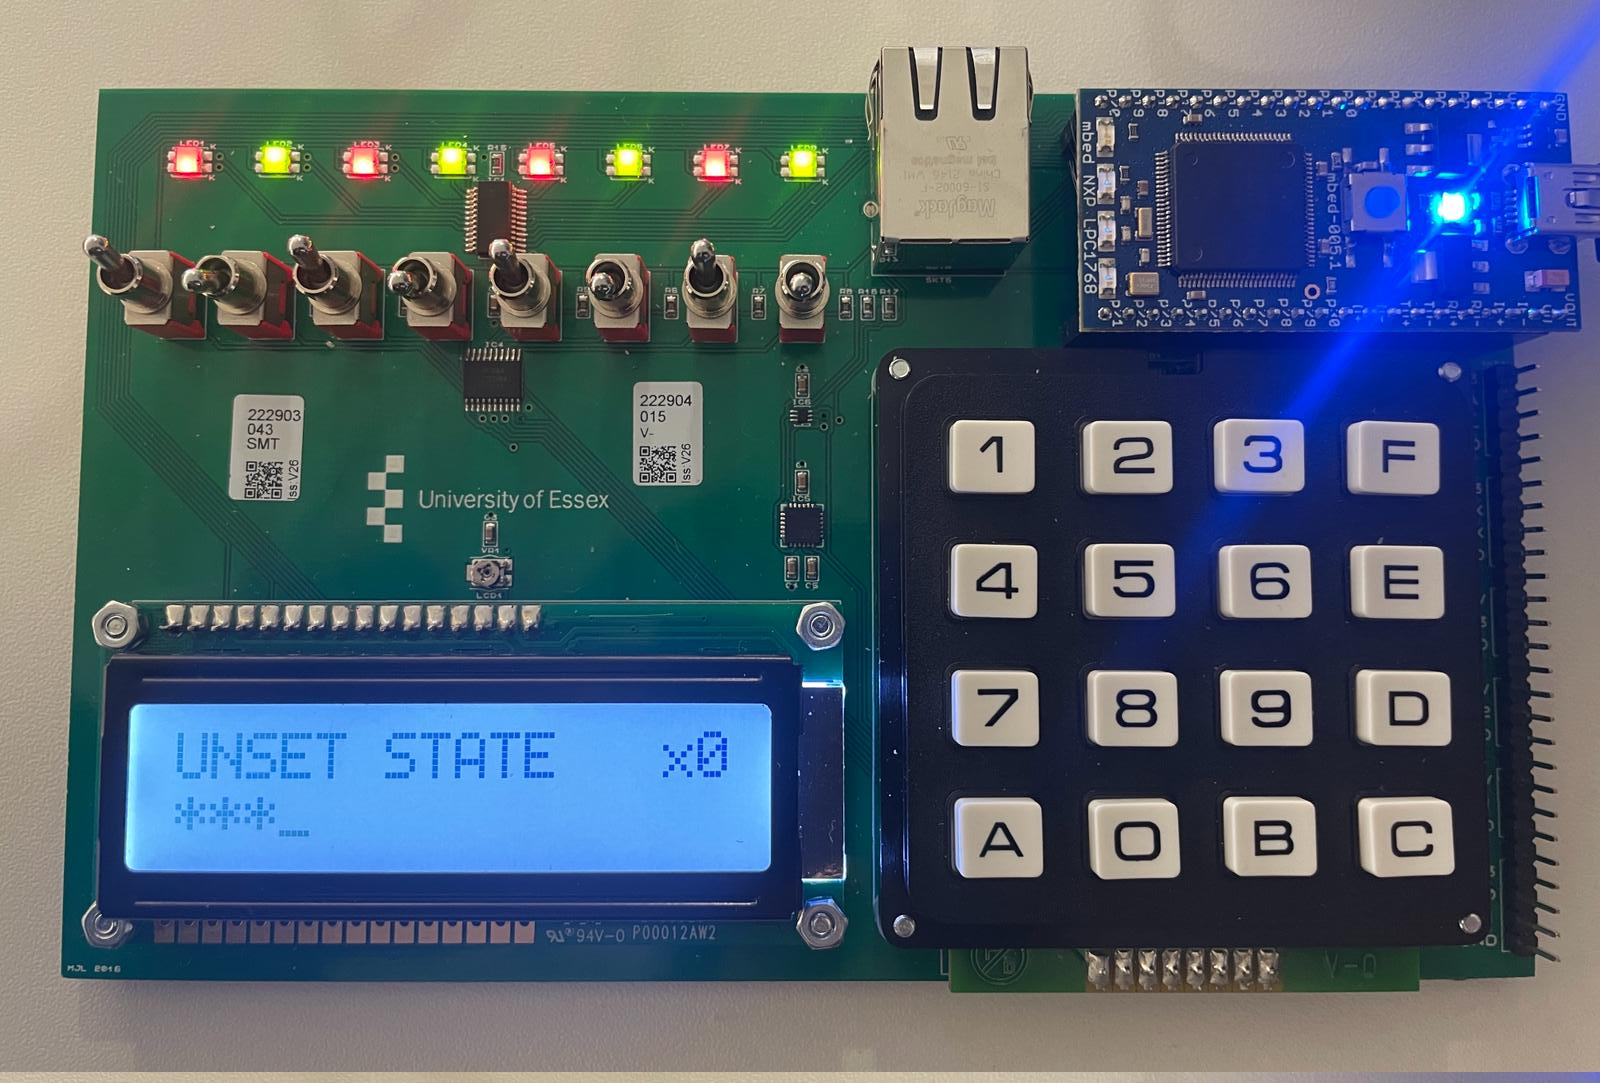
\includegraphics[scale = 0.3]{hardware.jpeg}
  \caption{\em Hardware used for the project}
  \label{fig:appendix1}
\end{figure}


}
% Appendix

\end{document}